\paragraph{三维基准结果。}

图~\ref{fig:3d_appendix_profiles}展示三维识别、开放问答与报告生成结果。CoEvoMed 在 M3D-VQA 五类任务中均取得最高准确率，总体准确率为80.11\%（11,048/13,791），类别宏平均为83.06\%；Med3DVLM-7B（Med3DVLM-Qwen-2.5-7B）~\citep{xin2025med3dvlm}的总体准确率为79.18\%。这些结果支持 CoEvoMed 在互补三维医学任务上的适用性。

\begin{figure}[!htbp]
\centering
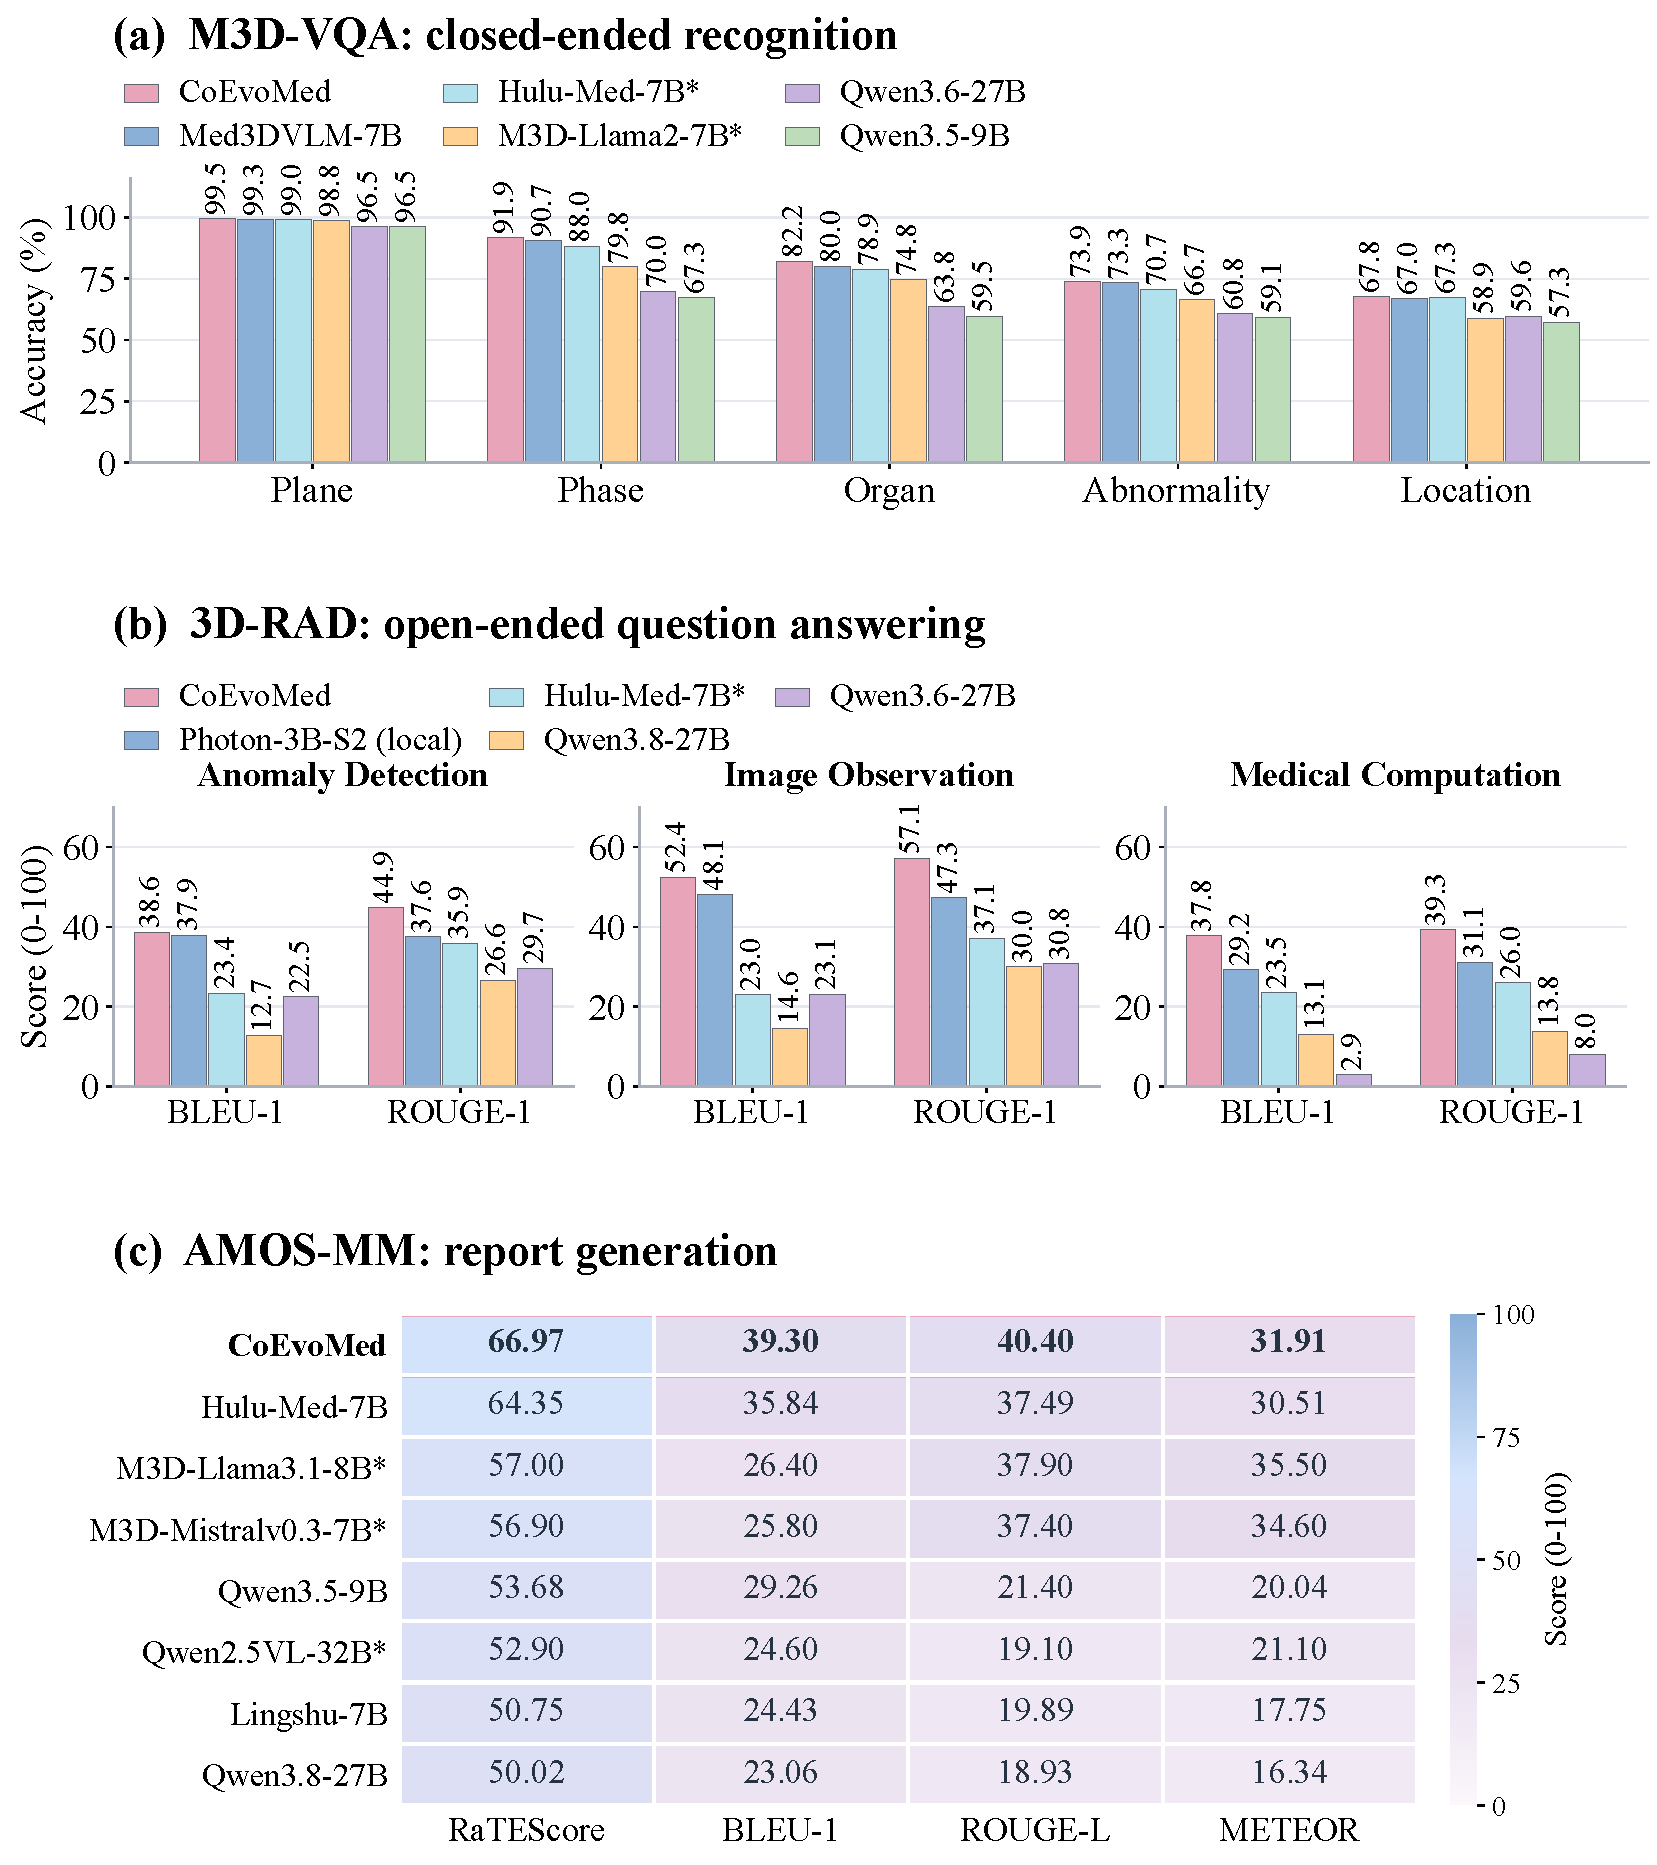
\includegraphics[width=0.84\linewidth]{figures/three_d_appendix_profiles.pdf}
\caption{三维基准细分结果。(a) M3D-VQA 五类闭合题的准确率。(b) 3D-RAD 三类开放任务的 BLEU-1 与 ROUGE-1；Photon 采用 S2 本地评测。(c) AMOS-MM 报告生成指标，标注原始数值并使用固定 0--100 色阶。各部分均展示 CoEvoMed 与排名靠前的可用基线：(a) 按类别平均准确率选取五个，(b) 按任务平均 ROUGE-1 选取四个，(c) 按 RaTEScore 选取七个。全部指标统一乘以100。星号标记 \citet{jiang2025hulumed} 的文献结果。}
\label{fig:3d_appendix_profiles}
\end{figure}
